\chapter{Solution}
\label{ch:solution}



\section{Ship Model}

\begin{figure} [h]
\centering
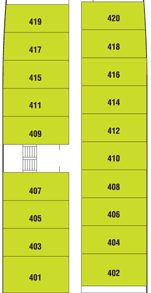
\includegraphics[angle=90]{images/rooms.png}
\caption{A small section of a ship deck}
\label{fig:rooms}
\end{figure}

\begin{figure} [h]
\centering
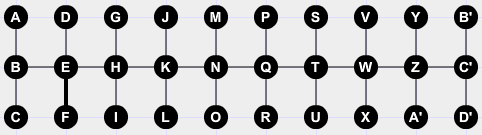
\includegraphics{images/simple.png}
\caption{The graph representing the ship deck}
\label{fig:simple}
\end{figure}

The ships are created from blueprints from ships currently in operation. They are modeled as graphs, nodes represents rooms and lines represents passages between rooms. Small rooms are represented by a single node as the layout of the room is fairly simplistic and the time it takes to move across the room is fairly predictable as long as the room is not crowded. Figure \ref{fig:rooms} shows a section of a ship deck with several rooms leading out into a hallway connected to a set of stairs. Figure \ref{fig:simple} shows a graph representing the same section. It is worth noting that while small rooms can be represented with a single node the hallway is represented by multiple nodes as a passenger exiting room 419 is far away from a passenger exiting room 401.

Complex or large rooms are represented by multiple interconnected nodes so each part of the room can be individually configured to better represent the room. Rooms like the dining room in the MS Reflection, as seen in figure \ref{fig:dining}, would need several nodes as the time it takes for the people close to the exit to evacuate are vastly different from the time it takes for the people sitting in the middle of the room to evacuate. Figure \ref{fig:complex} shows a representation of the dining room. 

\begin{figure} [h]
\centering
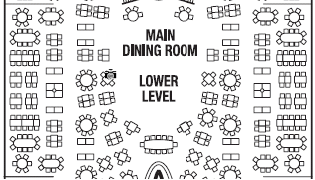
\includegraphics{images/Dining.png}
\caption{The dining room in the cruise ship MS Reflection}
\label{fig:dining}
\end{figure}

All rooms have a few characteristics associated with them. First is the room capacity, meaning the amount of people that can move across the room before they start to slow each other down. Second is the chance of death, this number will change over time as the fire spreads throughout the ship. Third is the type of room, for instance stairs, hallway, gift shop etc. Fourth is the size of the room, which in turn will determine the time it takes to traverse the room. Additionally there are a exit nodes where all passengers gather before lifeboat embarkation. These are the nodes the algorithms attempts to guide the passengers towards.

\begin{figure} [h]
\centering
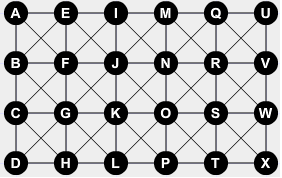
\includegraphics{images/complex.png}
\caption{A simple representation of the dining room of the MS Reflection}
\label{fig:complex}
\end{figure}

It became clear to us that using pathfinding algorithms to find the shortest route of small vessels were unnecessary as  there often would be only a single route to take and all passengers would be confined to one or two large areas where personnel easily could guide the passengers to safety. The algorithms are only helpful given multiple routes and rooms. We started off modeling one of the smaller cruise ships, MS Xpedition, and then went on to model larger vessels.

% Fire spreads based on

\section{Algorithm implementation}

When the fire starts either the fire system is able to track the position of the fire or the electric system have been compromised and the ship is in a dead ship condition where tracking the progress of the fire is impossible. If there are no information about the fire the on average safest possible route is the quickest one. 

\section{Human Behavior}

At the beginning of the simulation we assume that all passengers have access to a smart phone, which will show them the way out, and that they are following directions. Additionally, no passengers will start the simulation in a panicked state. However at certain time intervals a check is made to determine whether a passenger panics or not. Close proximity to fire, a high density of passengers or other panicked passengers increase the chance that they themselves will panic. When in a panicked state the passengers run out of the ship the same way they walked into it. Even if that path is significantly more dangerous.

Passengers with family members onboard the ship can enter a search state where they walk in a random pattern searching for family members until they find them, at which point they can resume following directions. The passengers can spot family members within their own node and any adjacent nodes. Family members that are not in a search state will also group up if they are within spotting range. In this case the family member that is further along the escape path will wait for the other family member to catch up.

Furthermore, family members will stick together and the algorithms will make no attempts to split up a family and send them in multiple directions. Thus whenever a passenger is moved the program checks if a family member is close-by, and if so they are moved in the same direction.



